\subsection{Heat Maps}
	This section will cover all the aspects of the heat maps use case (Figure \ref{HeatMapUseCase}). This use case is chosen as it is a vital part of the entire system. The data that is recorded will be used to create the heat maps that can then later be used to analyse the data and be used for future uses.
	\newline
	\begin{figure}[!ht]
		\centering
		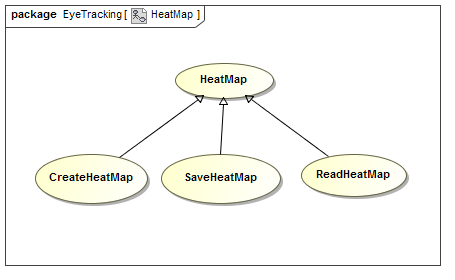
\includegraphics[scale=0.5]{Diagrams/Use_Case_Diagram__HeatMap.png}
		\caption{Heat Map Use Case}
		\label{HeatMapUseCase}
	\end{figure}
	

	The following sub use cases are included in this use case:
	\subsubsection{CreateHeatMap}
The create heat map use case deals with the creation of the heat map from the recorded data. The heat map shows where on the media item has been viewed the most by the user(s).
	\begin{itemize}
		\item Pre-condition: Eye tracking data must be already recorded.
		\item Post-condition: Heat-map of the data is created.
		\item Request Data Structure: Raw information recorded by eye tracking camera.
		\item Return data Structure: Heat-map is created
	\end{itemize}
	\begin{figure}[!ht]
		\centering
		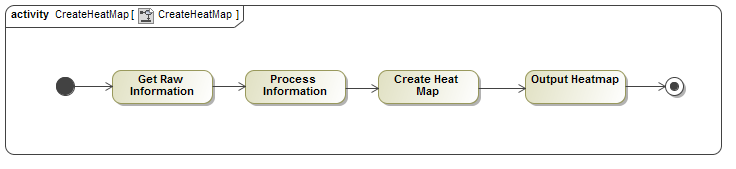
\includegraphics[scale=0.5]{Diagrams/Activity_Diagram__CreateHeatMap__CreateHeatMap.png}
		\caption{Create Heat Map Activity}
	\end{figure}
	
	\subsubsection{ReadHeatMap}
	This use case deals with the viewing of heat-maps from their recorded data. Once the heat-map is created the users will be able to see the heat-map and view the data.
	\begin{itemize}
		\item Pre-condition: Heat-map must have been created.
		\item Post-condition: Heat-map of the data is viewable and can be further analysed.
		\item Request Data Structure: The created heat-map.
		\item Return Data Structure: Heat-map is viewable to the user(s).
	\end{itemize}
	
	\begin{figure}[!ht]
		\centering
		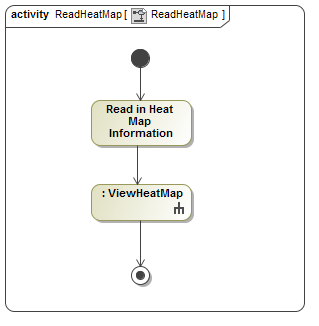
\includegraphics[scale=0.5]{Diagrams/Activity_Diagram__ReadHeatMap__ReadHeatMap.png}
		\caption{Read Heat Map Activity}
	\end{figure}
	
	\subsubsection{SaveHeatMap}
	This use case deals with the saving of heat-maps that are created from their respective recorded data. The heat-map will be saved on the users computer to be viewed at a later date. This will save only the heat-map which can later be saved onto a model at a later date.
	\begin{itemize}
		\item Pre-condition: Raw information must have already been recorded so that new heat-map can be created.
		\item Post-condition: Heat-map of the data is saved.
		\item Request Data Structure: Raw eye tracking information
		\item Return Data Structure: Heat-map is saved.
	\end{itemize}
	
	\begin{figure}[!ht]
		\centering
		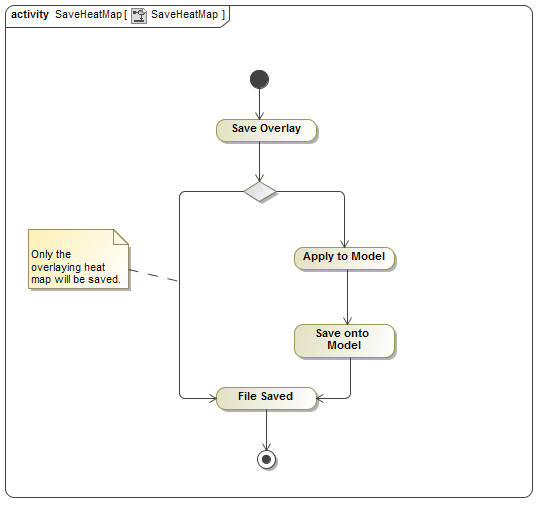
\includegraphics[scale=0.5]{Diagrams/Activity_Diagram__SaveHeatMap__SaveHeatMap.png}
		\caption{Save Heat Map Activity}
	\end{figure}
	
\subsection{Save Heat Maps}
	The saving of the heat-maps provides important functionality to the system as it will allow the users to save the data which can later be used to either continue research or to compare data.The heat-map will serve as an overlay for the media type and be placed over the media model. The saving of heat maps can be divided into three subsections, namely SaveHeatMapOntoModel3D, SaveHeatMapOntoModelVideo and SaveHeatMapOntoModel2D.
	\newline
	
	\begin{figure}[!ht]
		\centering
		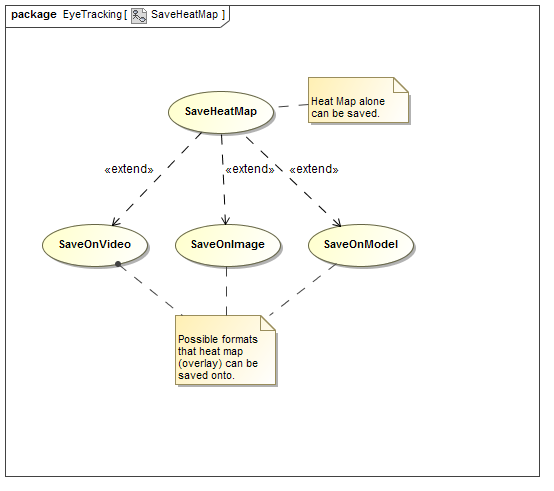
\includegraphics[scale=0.5]{Diagrams/Use_Case_Diagram__SaveHeatMap.png}\newline
		\caption{Save Heat Map Use Case}
	\end{figure}		
		
	
	\subsubsection{SaveHeatMapOntoModel2D}
The heat-map that is created for a 2D model media type will be saved and applied to the 2D model to see the heat-map on top of the model to indicate what has been viewed the most by the user(s) test participants.
	\begin{itemize}
		\item Pre-condition: Eye tracking data must have already been recorded.
		\item Post-condition: Heat map of the data is viewable on the 2D model as an overlay.
		\item Request Data Structure: Raw eye tracking data.
		\item Return Data Structure: Heat map of the data is placed over the 2D Model.
	\end{itemize}
	\begin{figure}[!ht]
		\centering	
		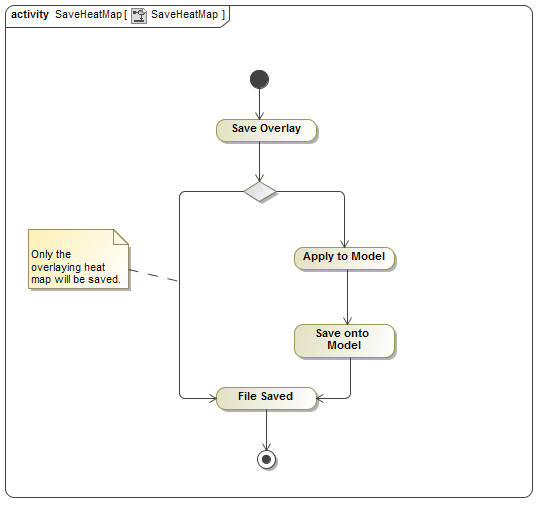
\includegraphics[scale=0.5]{Diagrams/Activity_Diagram__SaveHeatMap__SaveHeatMap.png}	
		\caption{Save on 2D Model Activity}
	\end{figure}

	\subsubsection{SaveHeatMapOntoModelVideo}
	The heat-map that is created for a video media type will be saved and then applied to the video to see the heat-map over the video to indicate what has been viewed the most by the users. The video model is spliced into images at either 30 or 60 frames per second of the video, the heat-maps can then be applied to the created images and recompiled into a new video.
	\begin{itemize}
		\item Pre-condition: Eye tracking data must have been recorded and video model must be available.
		\item Post-condition: New video is created with the heat-map on top of it.
		\item Request Data Structure: Video and raw information of recording.
		\item Return Data Structure: Heat-map of the data is placed over each frame of the video.
	\end{itemize}
	\begin{figure}[!ht]
		\centering	
		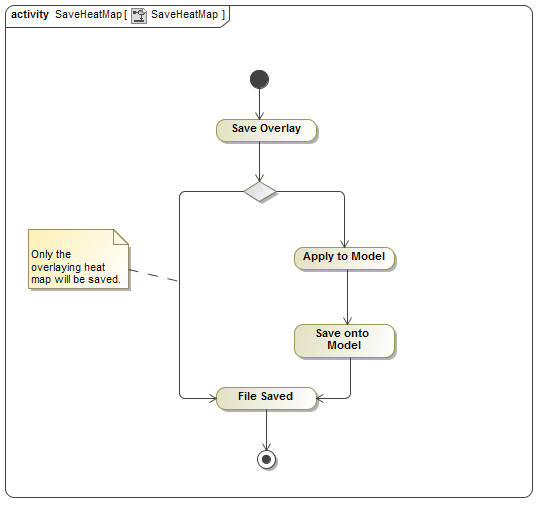
\includegraphics[scale=0.5]{Diagrams/Activity_Diagram__SaveHeatMap__SaveHeatMap.png}	
		\caption{Save on Video Model Activity}
	\end{figure}

	\subsubsection{SaveHeatMapOntoModel3D}
	The 3D model will have multiple images of it created from different angles Each created image can then have a heat-map placed over it.
	\begin{itemize}
		\item Pre-condition: Eye tracking data must have already been recorded and 3D model must be available for the creation of images.
		\item Post-condition: Heat-map of the data is viewable on the 3D model as an overlay.
		\item Request Data Structure: Recorded eye tracking information.
		\item Return Data Structure: Heat-map of the data is placed over each image of the 3D model.
	\end{itemize}
	\begin{figure}[!ht]
		\centering	
		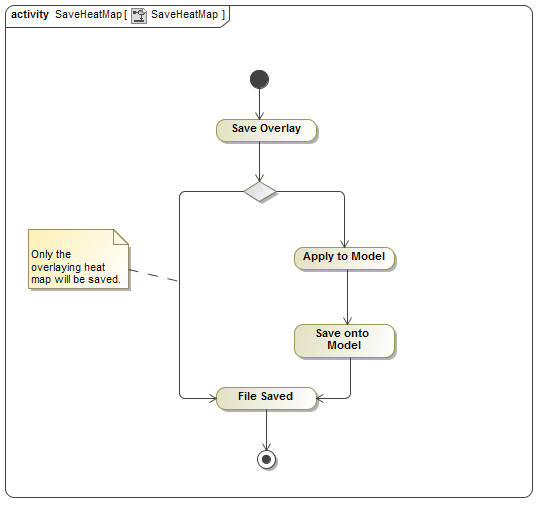
\includegraphics[scale=0.5]{Diagrams/Activity_Diagram__SaveHeatMap__SaveHeatMap.png}	
		\caption{Save on 3D Model Activity}
	\end{figure}
	
	%============================================================================%
	
\subsection{Gaze Point Maps}
	This section will cover all the aspects of the Gaze Point Map use case (Figure \ref{GazePointUseCase}). Gaze point maps track where the user is looking but specifies the order in which their respective gaze moves from one location to another. This use case forms an added extra to the user and can be used to further analyse information and data that has been recorded. The data that is recorded will be used to create the gaze point that can then later be used to analyse the data and be used for future uses.
	\newline
	\begin{figure}[!ht]
		\centering
		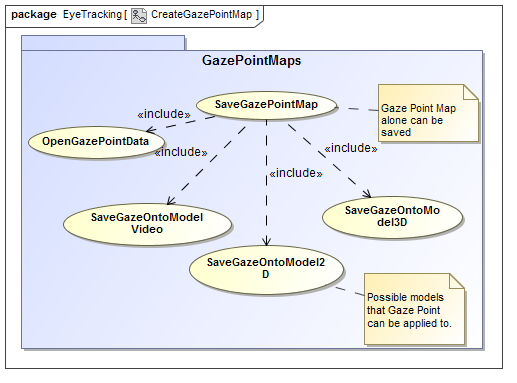
\includegraphics[scale=0.5]{Diagrams/Use_Case_Diagram__CreateGazePointMap.png}
		\caption{Gaze Point Use Case}
		\label{GazePointUseCase}
	\end{figure}
	

	The following sub use cases are included in this use case:
	\subsubsection{CreateGazePointMap}
The create gaze point activity deals with the creation of the gaze point maps from the recorded data. The gaze point map shows the order and length in which the subject views the model.
	\begin{itemize}
		\item Pre-condition: Eye tracking data must be already recorded.
		\item Post-condition: Gaze point map of the data is created.
		\item Request Data Structure: Raw information recorded by eye tracking camera.
		\item Return data Structure: Gaze point map is created
	\end{itemize}
	\begin{figure}[!ht]
		\centering
		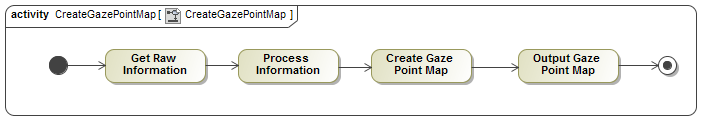
\includegraphics[scale=0.5]{Diagrams/Activity_Diagram__CreateGazePointMap__CreateGazePointMap.png}
		\caption{Create Gaze Point Map Activity}
	\end{figure}
	
	\subsubsection{ReadGazePointMap}
	This activity deals with the viewing of gaze point maps from their recorded data. Once the gaze point maps have been created the users will be able to see the gaze point maps and view the data.
	\begin{itemize}
		\item Pre-condition: Gaze point map must have been created.
		\item Post-condition: Gaze point map of the data is viewable and can be further analysed.
		\item Request Data Structure: The created gaze point map.
		\item Return Data Structure: Gaze point map is viewable to the user(s).
	\end{itemize}
	
	\begin{figure}[!ht]
		\centering
		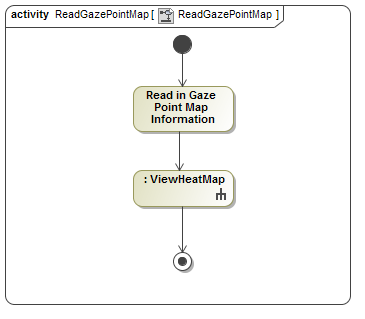
\includegraphics[scale=0.5]{Diagrams/Activity_Diagram__ReadGazePointMap__ReadGazePointMap.png}
		\caption{Read Gaze Point Map Activity}
	\end{figure}
	
	\subsubsection{SaveGazePointMap}
	This activity deals with the saving of gaze point map that are created from their respective recorded data. The gaze point map will be saved on the users computer to be viewed at a later date. This will save only the gaze point map which can later be saved onto a model at a later date.
	\begin{itemize}
		\item Pre-condition: Raw information must have already been recorded so that new gaze point map can be created.
		\item Post-condition: Gaze point map of the data is saved.
		\item Request Data Structure: Raw eye tracking information
		\item Return Data Structure: Gaze point map is saved.
	\end{itemize}
	
	\begin{figure}[!ht]
		\centering
		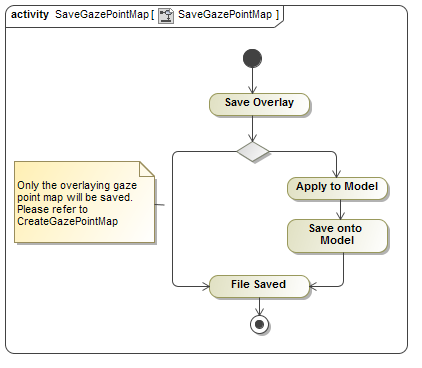
\includegraphics[scale=0.5]{Diagrams/Activity_Diagram__SaveGazePointMap__SaveGazePointMap.png}
		\caption{Save Gaze Point Map Activity}
	\end{figure}
	
\subsection{Save Gaze Point Maps}
	The saving of the gaze point map provides important functionality to the system as it will allow the users to save the data which can later be used to either continue research or to compare data.The gaze point map will serve as an overlay for the media type and be placed over the media model. The saving of gaze point map can be divided into three subsections, namely SaveGazeMapOntoModel3D, SaveGazeMapOntoModelVideo and SaveGazeMapOntoModel2D.
	\newline
	
	\begin{figure}[!ht]
		\centering
		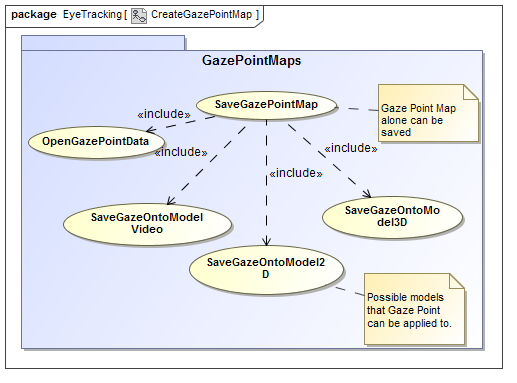
\includegraphics[scale=0.5]{Diagrams/Use_Case_Diagram__CreateGazePointMap.png}\newline
		\caption{Save Gaze Point Map Use Case}
	\end{figure}		
		
	
	\subsubsection{SaveGazeMapOntoModel2D}
The gaze point map that is created for a 2D model media type will be saved and applied to the 2D model to see the gaze point map on top of the model to indicate what has been viewed the most by the user(s) test participants.
	\begin{itemize}
		\item Pre-condition: Eye tracking data must have already been recorded.
		\item Post-condition: Gaze point map of the data is viewable on the 2D model as an overlay.
		\item Request Data Structure: Raw eye tracking data.
		\item Return Data Structure: Gaze point map of the data is placed over the 2D Model.
	\end{itemize}
	\begin{figure}[!ht]
		\centering	
		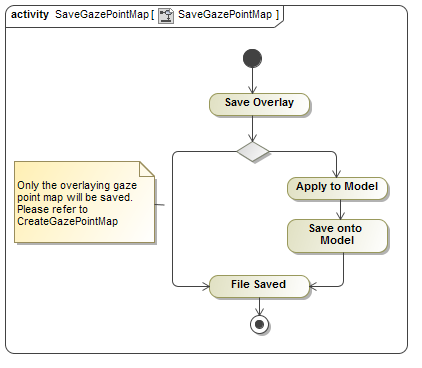
\includegraphics[scale=0.5]{Diagrams/Activity_Diagram__SaveGazePointMap__SaveGazePointMap.png}	
		\caption{Save on 2D Model Activity}
	\end{figure}

	\subsubsection{SaveGazeMapOntoModelVideo}
	The gaze point map that is created for a video media type will be saved and then applied to the video to see the gaze point map over the video to indicate what has been viewed the most by the users. The video model is spliced into images at either 30 or 60 frames per second of the video, the gaze point map can then be applied to the created images and recompiled into a new video.
	\begin{itemize}
		\item Pre-condition: Eye tracking data must have been recorded and video model must be available.
		\item Post-condition: New video is created with the gaze point map on top of it.
		\item Request Data Structure: Video and raw information of recording.
		\item Return Data Structure: Gaze point map of the data is placed over each frame of the video.
	\end{itemize}
	\begin{figure}[!ht]
		\centering	
		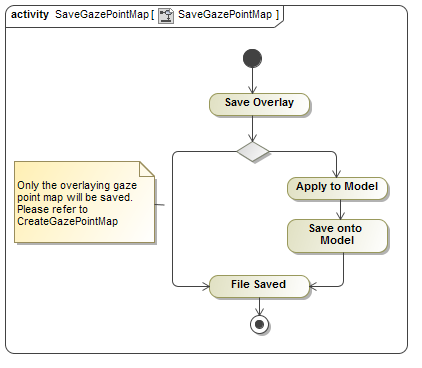
\includegraphics[scale=0.5]{Diagrams/Activity_Diagram__SaveGazePointMap__SaveGazePointMap.png}	
		\caption{Save on Video Model Activity}
	\end{figure}

	\subsubsection{SaveGazeMapOntoModel3D}
	The 3D model will have multiple images of it created from different angles Each created image can then have a gaze point map placed over it.
	\begin{itemize}
		\item Pre-condition: Eye tracking data must have already been recorded and 3D model must be available for the creation of images.
		\item Post-condition: Gaze point map of the data is viewable on the 3D model as an overlay.
		\item Request Data Structure: Recorded eye tracking information.
		\item Return Data Structure: Gaze point map of the data is placed over each image of the 3D model.
	\end{itemize}
	\begin{figure}[!ht]
		\centering	
		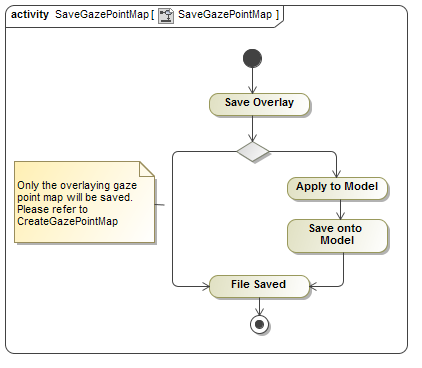
\includegraphics[scale=0.5]{Diagrams/Activity_Diagram__SaveGazePointMap__SaveGazePointMap.png}	
		\caption{Save on 3D Model Activity}
	\end{figure}	
	
	%============================================================================%
		
\subsection{Models}
This section details all the different types of media or models that heat-maps can be created for and saved onto. There are three types of models, namely Video, 2D and 3D. The heat maps are created based on the models and their types.
\newline
\begin{figure}[!ht]
	\centering	
	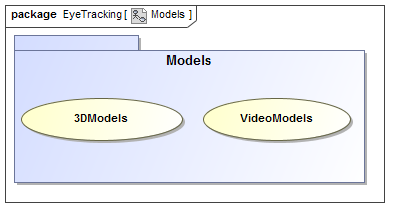
\includegraphics[scale=0.5]{Diagrams/Use_Case_Diagram__Models.png}
	\caption{Models Use Case}
\end{figure}
	
	\subsubsection{3D Models}
	3D Models will be opened and rendered by the system, and will then be made viewable to the user. The model will have images created of it at multiple angles. The heat-map can then be saved onto the models individual images as well as opened as the stand alone heat maps of each image.
	\newline
	\begin{figure}[!ht]
		\centering
		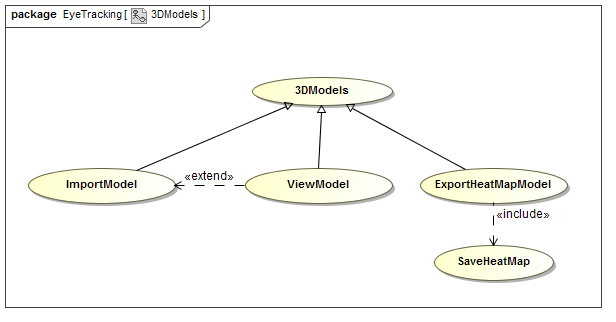
\includegraphics[scale=0.5]{Diagrams/Use_Case_Diagram__3DModels.png}
		\caption{3D Models Use Case}
	\end{figure}
	
	\begin{enumerate}
		\item{ImportModel}
		\newline
		This will allow for a 3D model media type to be imported into the system for further processing. The imported model can be used for recording data once the relevant images have been created and creating a relevant heat-map based on it which can then be applied to it at a later stage.
		\begin{itemize}
			\item Pre-condition: 3D model must exist.
			\item Post-condition: Images can be created and recording can be done on the model.
			\item Request Data Structure: The 3D model that user wishes to preform eye tracking on.
			\item Return Data Structure: Images of model will be created and returned.
		\end{itemize}
		
		\begin{figure}[!ht]
			\centering
			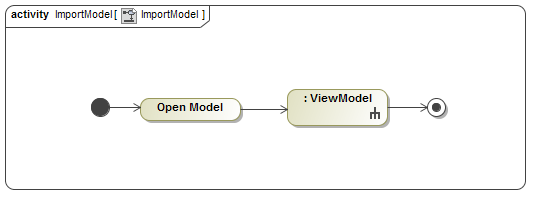
\includegraphics[scale=0.5]{Diagrams/Activity_Diagram__ImportModel__ImportModel.png}
			\caption{Import 3D Model Activity}
		\end{figure}
	
		\item{ViewModel}
		Once the model is imported the model and images created, the will be available for viewing and further processing decided by the user.
		\begin{itemize}
			\item Pre-condition: 3D model must have been imported and images created.
			\item Post-condition: The 3D model images are viewable and can be recorded on.
			\item Request Data Structure: The 3D models images.
			\item Return Data Structure: Viewable 3D model images.
		\end{itemize}
		\begin{figure}[!ht]
			\centering
			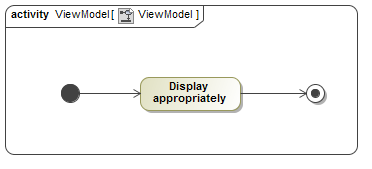
\includegraphics[scale=0.5]{Diagrams/Activity_Diagram__ViewModel__ViewModel.png}
		\caption{View 3D Model Activity}
		\end{figure}
		
		\item{ExportHeatMapModel}
		The exported model will have the heat-map applied to it which can then be exported as a new images of the 3D model so that it can be viewed or used at a later date by the user. 
		\begin{itemize}
			\item Pre-condition: Heat-map must be created and Model Imported.
			\item Post-condition: Exported model With heat-map on it to be viewed.
			\item Request Data Structure: The eye tracking data must have been recorded and 3D model available
			\item Return Data Structure: Model with heat-map applied.
		\end{itemize}
		
		\item{Export3DModelImages}
		The model will have images created from various angles of the model. These images can then be used for recording.
		\begin{itemize}
			\item Pre-condition: Selected model must be available.
			\item Post-condition: Images will be created of model.
			\item Request Data Structure: The selected model.
			\item Return Data Structure: Images of 3D model.
		\end{itemize}
		
		\begin{figure}[!ht]
			\centering
			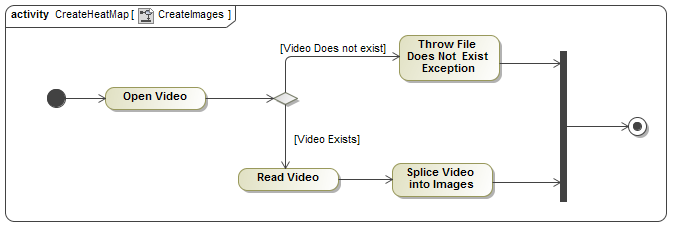
\includegraphics[scale=0.5]{Diagrams/Activity_Diagram__CreateHeatMap__CreateImages.png}
			\caption{Create 3D Model Images Activity}
		\end{figure}
	\end{enumerate}

	\subsubsection{2D Models}
	2D models will typically refer to images but can also refer to any media that is does not show a third dimension of movement but for the scope of this project will only refer to images. The heat-map can then be created and applied to the image.
	\newline
	\begin{figure}[!ht]
		\centering
		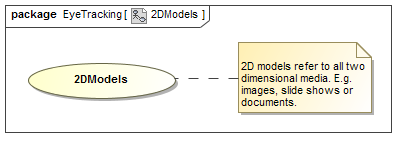
\includegraphics[scale=0.5]{Diagrams/Use_Case_Diagram__2DModels.png}
		\caption{2D Models Use Case}
	\end{figure}
	\begin{enumerate}
		\item{ImportModel}
		\newline
		The 2D models can be imported into the system which can then be process further by the user. The imported model can then have recordings done and heat maps created for it. 
		\begin{itemize}
			\item Pre-condition: The 2D model must exist, a image preferable.
			\item Post-condition: Recording can be done on the model.
			\item Request Data Structure: The desired 2D model.
			\item Return Data Structure: Rendered image is imported.
		\end{itemize}
		
		\begin{figure}[!ht]
			\centering
			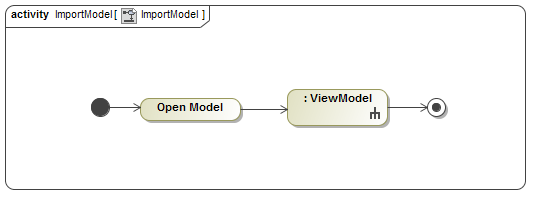
\includegraphics[scale=0.5]{Diagrams/Activity_Diagram__ImportModel__ImportModel.png}
			\caption{Import 2D Model Activity}
		\end{figure}
	
		\item{ViewModel}
		Once the model is imported the users can view the model and eye tracking can then be applied on the model. The model can the be processed further as the user sees fit.
		\begin{itemize}
			\item Pre-condition: The 2D model (image) must have been imported.
			\item Post-condition: Image is viewable and can be recorded on.
			\item Request Data Structure: The selected model image.
			\item Return Data Structure: Viewable image.
		\end{itemize}
		
		\begin{figure}[!ht]
			\centering
			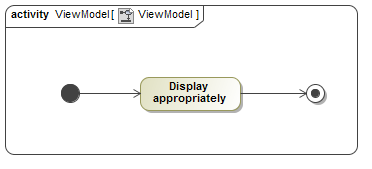
\includegraphics[scale=0.5]{Diagrams/Activity_Diagram__ViewModel__ViewModel.png}
			\caption{View 2D Model Activity}
		\end{figure}
	
		\item{ExportHeatMapModel}
		The exported model will have the heat map applied to it which can then be exported as a new 2D model so that it can be viewed or used at a later date by the user.  
		\begin{itemize}
			\item Pre-condition: The eye data must have been recorded and model imported.
			\item Post-condition: Exported model with heat-map on it to be viewed.
			\item Request Data Structure: Recorded eye data and imported model.
			\item Return Data Structure: Model with heat map.
		\end{itemize}
		
		\begin{figure}[!ht]
			\centering
			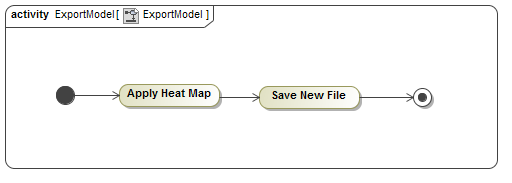
\includegraphics[scale=0.5]{Diagrams/Activity_Diagram__ExportModel__ExportModel.png}
			\caption{Export 2D Model Activity}
		\end{figure}
	
	\end{enumerate}
		
		
	\subsubsection{Video Models}
	A video can be easily imported into the system. Eye tracking can then be done to the video model and the recorded data can be stored. The data can then be used to create a heat-map that can then be applied to the video second by second.
	\newline
	
	\begin{figure}[!ht]
		\centering
		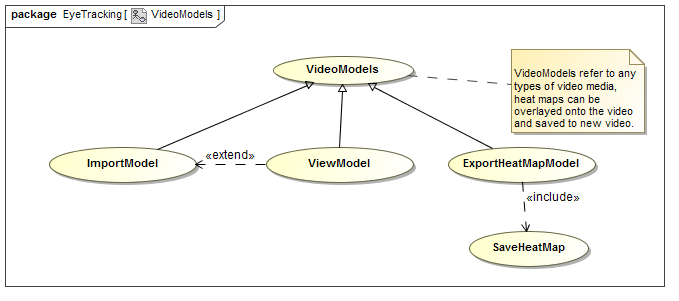
\includegraphics[scale=0.5]{Diagrams/Use_Case_Diagram__VideoModels.png}
		\caption{Video Models Use Case}
	\end{figure}
	
		\begin{enumerate}
			\item{ImportModel}
			\newline
			The video models can be imported into the system which can then be processed further by the user. The imported model can then have recordings done and heat maps created for it. Heat maps that will be recorded will show a second by second representation of the heat map data.
			\begin{itemize}
				\item Pre-condition: Desired video must exist.
				\item Post-condition: Recording can be done on the video.
				\item Request Data Structure: The video model.
				\item Return Data Structure: Rendered video is imported.
			\end{itemize}
			
			\begin{figure}[!ht]
				\centering
				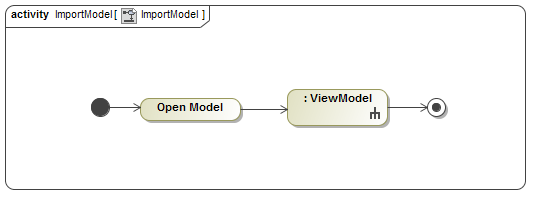
\includegraphics[scale=0.5]{Diagrams/Activity_Diagram__ImportModel__ImportModel.png}
				\caption{Import Video Model Activity}
			\end{figure}
			
			\item{ViewModel}
Once the model is imported the users can view the model and eye tracking can then be applied on the 	model. The model can the be processed further as the user sees fit.
			\begin{itemize}
				\item Pre-condition: Desired video model must be available.
				\item Post-condition: Video can be played and recordings taken.
				\item Request Data Structure: Requested video.
				\item Return Data Structure: Playable video.
			\end{itemize}
			\begin{figure}
				\centering
				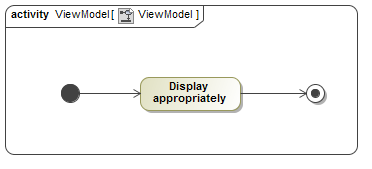
\includegraphics[scale=0.5]{Diagrams/Activity_Diagram__ViewModel__ViewModel.png}
				\caption{View Video Model Activity}
			\end{figure}
			
			
			
			\item{ExportHeatMapModel}
			The exported model will have the heat-map applied to it which can then be exported as a new video model so that it can be viewed or used at a later date by the user. The exported video model will have the heat map recorded onto the original video and saved in the appropriate format.
			\begin{itemize}
				\item Pre-condition: Eye tacking data must have been recorded and desired video imported.
				\item Post-condition: New video with heat-map overlay will be saved..
				\item Request Data Structure: Eye tracking data as well as the desired model.
				\item Return Data Structure: Video with heat map is saved.
			\end{itemize}
		\begin{figure}[!ht]
			\centering
			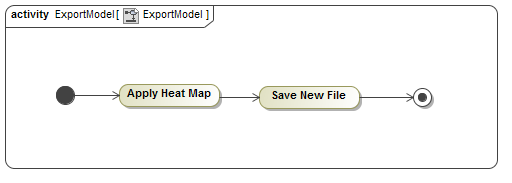
\includegraphics[scale=0.5]{Diagrams/Activity_Diagram__ExportModel__ExportModel.png}
			\caption{Export 3D Model Activity}
		\end{figure}
	
		\end{enumerate}
		
%=========================================================%		
\subsection{Raw Information}
When recording happens on the system the raw information is saved. The raw information is important as it forms the basis for creating heat maps and statistics for specific models. The raw information is can be saved on the system and processed further by the user. The raw information can then be read as the raw data or put into a statistical formats.
\newline

\begin{figure}[!ht]
	\centering
	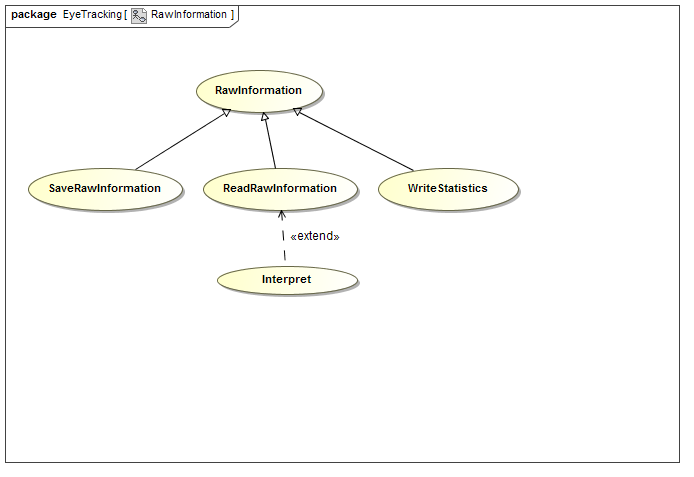
\includegraphics[scale=0.5]{Diagrams/Use_Case_Diagram__RawInformation.png}
	\caption{Raw Information Use Case}
\end{figure}
	
	\subsubsection{SaveRawInformation}
When recording is done on the media the raw information will need to be saved so that it can be used at a later stage. This raw information can then be reopened later for the relevant model and used by user for further processing and interpretation.
\begin{itemize}
\item Pre-condition: Recording on a media type must have already taken place.
\item Post-condition: Data is saved and can be used later.
\item Request Data Structure: Incoming x- and y-axis data coming form the Eye Tribe recording server.
\item Return Data Structure: The recorded eye tracking data text file is created.
\end{itemize}

\begin{figure}[!ht]
	\centering
	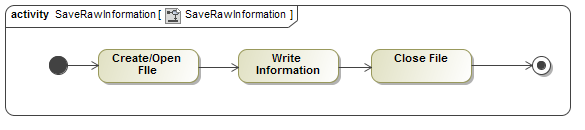
\includegraphics[scale=0.5]{Diagrams/Activity_Diagram__SaveRawInformation__SaveRawInformation.png}
	\caption{Save Raw Information Activity}
\end{figure}

	\subsubsection{ReadRawInformation}
Data can be read from a previously saved file. This will allow the user to import the raw information for the relevant model which can then be used for comparison or further processing.
\begin{itemize}
\item Pre-condition: Recorded data must have been saved in a text file.
\item Post-condition: Data can now be used to create heat-maps and statistics.
\item Request Data Structure: The recorded eye tracking data text file.
\item Return Data Structure: Data array with all data points that can then be further processed by application.
\end{itemize}

\begin{figure}[!ht]
	\centering
	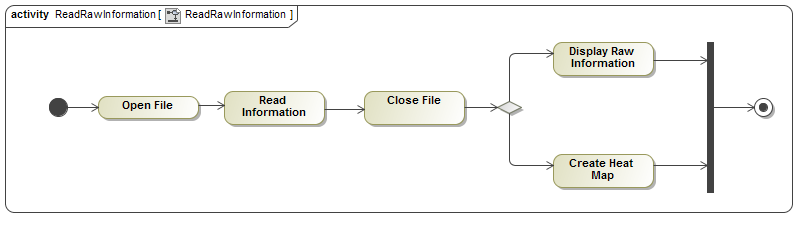
\includegraphics[scale=0.5]{Diagrams/Activity_Diagram__ReadRawInformation__ReadRawInformation.png}
	\caption{Read Raw Information Activity}
\end{figure}
	
	\subsubsection{CreateStatistics}
The writing of statistics is part of the Statistics use-case and all information can be found there regarding the sub use case

	
	
\subsection{Statistics}
Statistics on all the data will be collected and will then be used to make a statistical page based off the model that can be analysed and then it can be easily compared at any time.
\newline
\begin{figure}[!ht]
	\centering
	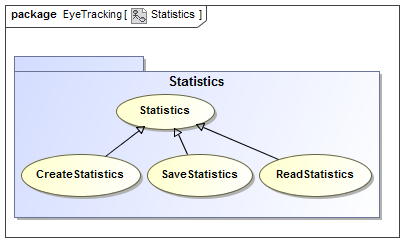
\includegraphics[scale=0.5]{Diagrams/Use_Case_Diagram__Statistics.png}
	\caption{Statistics Use Case}
	\end{figure}
	
		\subsubsection{CreateStatistics}
Using the recorded data we can create statistical data which can then be used for analysis. This data can then be viewed or used to compared data.
\begin{itemize}
\item Pre-condition: Recorded data must exist.
\item Post-condition: Data is turned into statistical data.
\item Request Data Structure: Text file containing recorded data.
\item Return Data Structure: Statistics will be created.
\end{itemize}

\begin{figure}[!ht]
	\centering
	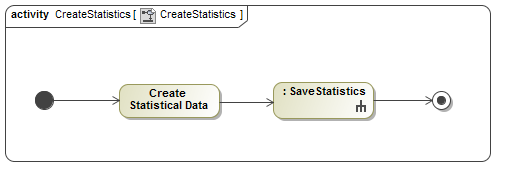
\includegraphics[scale=0.5]{Diagrams/Activity_Diagram__CreateStatistics__CreateStatistics.png}
	\caption{Create Statistics Activity}
	\end{figure}
	
		\subsubsection{SaveStatistics}
The statistical data can be saved into a file so that they can be printed out and be used further by users. This will take all created statistical data and save it into a pdf, excel or csv file.
\begin{itemize}
\item Pre-condition: Statistical data must exist.
\item Post-condition: Data is put into a report.
\item Request Data Structure: Created statistical data.
\item Return Data Structure: Save report in pdf, excel or csv format.
\end{itemize}

\begin{figure}[!ht]
	\centering
	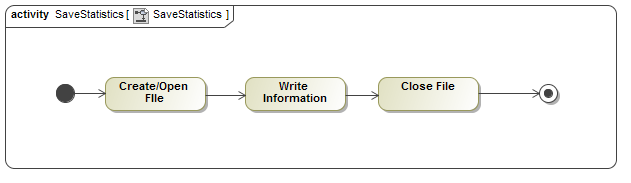
\includegraphics[scale=0.5]{Diagrams/Activity_Diagram__SaveStatistics__SaveStatistics.png}
	\caption{Save Statistics Activity}
	\end{figure}
	
\subsection{Record Eyes}
The recording of the eyes will be done using the Eye Tribe camera or any other (compatible) eye tracking camera. The data recorded in this process will allow heat maps and statistics to be generated. The heat maps can then be turned into overlays for the appropriate media types. The record eye use case (Figure \ref{RecordEye}) makes use of sub use cases from other use cases that are listed below, such as SaveRawInformation. The recording of the information is important as this is used throughout the project and its functionality.
\newline

\begin{figure}[!ht]
	\centering 
	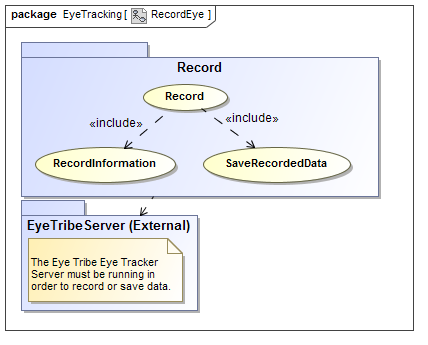
\includegraphics[scale=0.5]{Diagrams/Use_Case_Diagram__RecordEye.png}
	\caption{Record Eye Use Case}
	\label{RecordEye}
	\end{figure}
	
\subsubsection{RecordInformation}
The data will be recorded and saved into a text file which can be further processed and interpreted, which will then return the relevant information which can then be used to carry out functions in the system.
\begin{itemize}
\item Pre-condition: Calibration must have been previously completed and user must be viewing the specified media type, so that recording of data can take place.
\item Post-condition: Data is recorded about the eye movements and saved by another function.
\item Request Data Structure: N/A.
\item Return Data Structure: Raw data in x and y co-ordinates will be returned.
\end{itemize}

\begin{figure}[!ht]
	\centering
	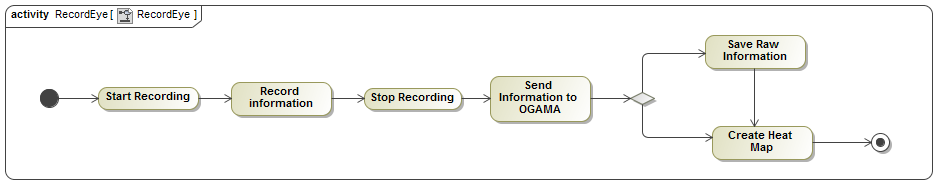
\includegraphics[scale=0.5]{Diagrams/Activity_Diagram__RecordEye__RecordEye.png}
	\caption{Record Eye Activity}
	\end{figure}

